\documentclass[aps,twocolumn,secnumarabic,balancelastpage,amsmath,amssymb,nofootinbib]{revtex4}
\usepackage{amsmath}
\usepackage{amssymb}
\usepackage{amsfonts}
\usepackage{chapterbib}
\usepackage{color}
\usepackage{graphics}
\usepackage[pdftex]{graphicx}
\usepackage{grffile}
\usepackage{longtable}
\usepackage{epsf}
\usepackage{bm}
\usepackage{tikz}
\usepackage{asymptote}
\usepackage{thumbpdf}
\usepackage{bbm}
\usepackage{amscd}
\usepackage{units}
\usepackage{textcomp}
\usepackage[utf8x]{inputenc}
\usepackage{feyn}
\usepackage{feynmp}
\usepackage[colorlinks=true]{hyperref}
\newcommand{\drelectron}[1]{\node at #1 [circle, draw, inner sep=0pt, minimum size=1pt] {\_}}

\newcommand{\ud}{\mathrm{d}}
\newcommand{\ue}{\mathrm{e}}
\newcommand{\ui}{\mathrm{i}}
\newcommand{\res}{\mathrm{Res}}
\newcommand{\Tr}{\mathrm{Tr}}
\newcommand{\dsum}{\displaystyle\sum}
\newcommand{\dprod}{\displaystyle\prod}
\newcommand{\dlim}{\displaystyle\lim}
\newcommand{\dint}{\displaystyle\int}
\newcommand{\fsno}[1]{{\!\not\!{#1}}}
\newcommand{\eqar}[1]
{
  \begin{align*}
    #1
  \end{align*}
}
\newcommand{\eqarn}[1]
{
  \begin{align}
    #1
  \end{align}
}
\newcommand{\texp}[2]{\ensuremath{{#1}\times10^{#2}}}
\newcommand{\dexp}[2]{\ensuremath{{#1}\cdot10^{#2}}}
\newcommand{\eval}[2]{{\left.{#1}\right|_{#2}}}
\newcommand{\paren}[1]{{\left({#1}\right)}}
\newcommand{\lparen}[1]{{\left({#1}\right.}}
\newcommand{\rparen}[1]{{\left.{#1}\right)}}
\newcommand{\abs}[1]{{\left|{#1}\right|}}
\newcommand{\sqr}[1]{{\left[{#1}\right]}}
\newcommand{\crly}[1]{{\left\{{#1}\right\}}}
\newcommand{\angl}[1]{{\left\langle{#1}\right\rangle}}
\newcommand{\tpdiff}[4][{}]{{\paren{\frac{\partial^{#1} {#2}}{\partial {#3}{}^{#1}}}_{#4}}}
\newcommand{\tpsdiff}[4][{}]{{\paren{\frac{\partial^{#1}}{\partial {#3}{}^{#1}}{#2}}_{#4}}}
\newcommand{\pdiff}[3][{}]{{\frac{\partial^{#1} {#2}}{\partial {#3}{}^{#1}}}}
\newcommand{\diff}[3][{}]{{\frac{\ud^{#1} {#2}}{\ud {#3}{}^{#1}}}}
\newcommand{\psdiff}[3][{}]{{\frac{\partial^{#1}}{\partial {#3}{}^{#1}} {#2}}}
\newcommand{\sdiff}[3][{}]{{\frac{\ud^{#1}}{\ud {#3}{}^{#1}} {#2}}}
\newcommand{\tpddiff}[4][{}]{{\left(\dfrac{\partial^{#1} {#2}}{\partial {#3}{}^{#1}}\right)_{#4}}}
\newcommand{\tpsddiff}[4][{}]{{\paren{\dfrac{\partial^{#1}}{\partial {#3}{}^{#1}}{#2}}_{#4}}}
\newcommand{\pddiff}[3][{}]{{\dfrac{\partial^{#1} {#2}}{\partial {#3}{}^{#1}}}}
\newcommand{\ddiff}[3][{}]{{\dfrac{\ud^{#1} {#2}}{\ud {#3}{}^{#1}}}}
\newcommand{\psddiff}[3][{}]{{\frac{\partial^{#1}}{\partial{}^{#1} {#3}} {#2}}}
\newcommand{\sddiff}[3][{}]{{\frac{\ud^{#1}}{\ud {#3}{}^{#1}} {#2}}}

\begin{document}
\tikzstyle{every picture}+=[remember picture]
\title{Simulation of Raman sideband cooling with large Lamb-Dicke factor and high initial temperature}
\author{Yichao Yu}
\email{yuyichao@mit.edu}
\homepage{http://yyc-arch.org/}
\date{\today}
\affiliation{MIT Department of Physics}

\begin{abstract}
  It is usually believed that Raman sideband cooling requires a particle to be confined to much smaller than the optical wavelength, i.e. small Lamb-Dicke factor and low initial vibrational state, in order to suppress the heating from light scattering. In this paper, I will show with numerical simulation of the optical Bloch equation that by driving Raman transitions between vibrational states with $\delta n\gg1$, it is possible to preform Raman sideband cooling with a big Lamb-Dicke factor ($\eta=0.8$) and a high initial temperature $k_BT/\hbar\omega=30$.
\end{abstract}

\maketitle
%%%%%%%%%%%%%%%%%%%%%%%%%%%%%%%%%%%%%%%%%%%%%%%%%%%%%%%%%%%%%%%%%%
\section{Introduction}
Sideband cooling is a powerful technique for cooling confined particles, especially for ions in ion traps, to their ground states in both external and internal degrees of freedom. One of its variation, is also used in some experiment for cooling neutral atoms confined in an optical lattice\cite{sideband-cs-lattice} or a tightly focused tweezer optical dipole trap\cite{sideband-single-jila,sideband-single-cua}. Due to the heating from photon scattering, most of these experiments requires the particle to be confined to much smaller than an optical wavelength. Although this is possible to do for heavy atoms, e.g. Rubidium and Cesium, or ions, it is hard to get the same confinement for lighter neutral atoms like sodium.\\

Although the heating from optical pumping is faster with looser confinement, the strength of Raman transition to vibrational states much more than one level lower also increases ($\delta n\gg1$), which raises the possibility of faster cooling by driving Raman transition to take away more than one quanta of vibrational energy ($\hbar\omega$). In this paper, I am going to study the possibility of such cooling scheme using numerical stimulations and show that with carefully optimized cooling sequence, one can use this method to cool atoms with a relatively loose confinement and high initial temperature to its low vibrational states.

\section{Theory of Raman sideband cooling}
\subsection{Sideband and Lamb-Dicke factor}
When a particle is confined in a harmonic potential, the spectrum of the external degrees of freedom become a series of discrete harmonic oscillator levels ($\hbar\omega$) as oppose to a continuum for free particles ($p^2/2m$). The effect of the coupling between the external and internal degrees of freedom also becomes discrete. As a result, instead of the Doppler effect and the recoil shift, the coupling to the external harmonic oscillator levels splits each of the transitions of the particle to a set of sidebands separated by the trapping frequency. The strength of the coupling can be calculated from the recoil of the photon, i.e. the phase gradient of the electric magnetic field,
\eqarn{
  \frac{\Omega_{n,n'}}{\Omega}=&\abs{\langle n|\ue^{\ui kr}|n'\rangle}\\
  =&\abs{\langle n|\ue^{\ui \eta\paren{a^\dagger+a}}|n'\rangle}\label{lamb-dicke}
}
where $\Omega_{n,n'}$ is the Rabi frequency coupling two different vibrational states $n$ and $n'$, $\Omega$ is the original Rabi frequency for the internal transition, $k$ is the wave vector of the light, $a$ and $a^\dagger$ are the lowering and raising operators for the harmonic oscillator and $\eta$ is the Lamb-Dicke factor defined as,
\eqar{
  \eta=k\sqrt{\frac{\hbar}{2m\omega}}
}
We can easily see from the expression of the coupling strengh that in order to have strong couping between two levels, both of the harmonic oscillator wave functions must have a spatial extend comparable to the optical wavelength. Otherwise, the phase from the photon field will act as a global phase on the wavefunction and cannot create any coupling to other energy levels. The same expression also works for two-photon transitions, in which case the wave vector $k$ should be replaced by the difference between the wave vectors of the two photons.

\subsection{Raman Sideband Cooling}
Since the harmonic confinement turns the spectrum of external motion into discrete bands, one can drive transitions between these levels with narrow band lasers for cooling. This can be done with normal optical transition in an ion trap with a trapping frequency of several $MHz$ but is usually done with a narrow Raman transition for neutral atoms in an optical trap, hence the name Raman sideband cooling.\\

The Raman sideband cooling of atoms requires two ground states that can be coupled through a Raman transition. Examples of such states used in experiments include hyperfine states or different Zeeman levels in a magnetic field. The atoms first start in one of the ground states $|1\rangle$. Two Raman beams red detuned by $\delta n\omega$ to the original Raman resonance are used to transfer the atoms into the other ground state $|2\rangle$ at a vibrational state $\delta n$ levels lower. An optical pumping beam is then used to pump the atom in the state $|2\rangle$ back to state $|1\rangle$ and the cycle is repeated. In order for the cooling to work efficiently, the optical pumping beam must not introduce more heating (changes in vibrational levels) on average than the vibrational energy taken out by the Raman transition. This is usually done by tightly confine the particles and therefore decrease the probability of going into another vibrational level. However, if it is not practical to provide enough confinement in the experiment, e.g. for light atoms, one can also increasing the cooling effect from the Raman transition by using $\delta n>1$ and this is what I am going to study in the following sections.

\section{Simulation using Optical Bloch Equation}
\subsection{The system to simulate}
In order to study the Raman sideband cooling scheme, I am going to simulate a simple system, a single atom trapped in a tightly confined tweezer trap. It is similar to the ones realized recently in the experiment at JILA\cite{sideband-single-jila} and Harvard\cite{sideband-single-cua}. However, instead of using the heavy Rubidium atoms, the atom used in this simulation is the much lighter Soldium atom.\\

The simulation is going to be done on the cooling of the longitudinal degree of freedom for a soldium atom trapped in a optical dipole trap created by focusing a $3\text{mW}$ $\lambda=1064\text{nm}$ laser with numerical aperture $NA=0.55$. The Lamb-Dicke factor for the $D$ lines along the longitudinal direction is $\eta\approx0.8$. The two states used for the Raman transition are the $F=2, m_F=-2$ and $F=1, m_F=-1$ hyperfine states with dark state pumping with $\sigma^-$ light on the $D1$ line to pump atoms from $F=1, m_F=-1$ back to $F=2, m_F=-2$. The initial temperature of the atom in the trap is $T=30\hbar\omega/k_B\approx50\mu K$, which is closed to the temperature achievable by polarization gradient cooling for soldium.\\

In order to be closer to the real experimental condition, it also includes a $5\%$ heating effect from the optical pumping beam on the atoms in the dark state, which can come from the misalignment of the pumping beam with the magnetic field. The two Raman beams are sent in from radial and longitudinal directions instead of both in the more effecient longitudinal direction since one side of the axis may be blocked by the focusing lens for the optical dipole trap in the experiment.

\begin{figure}
  \begin{center}
    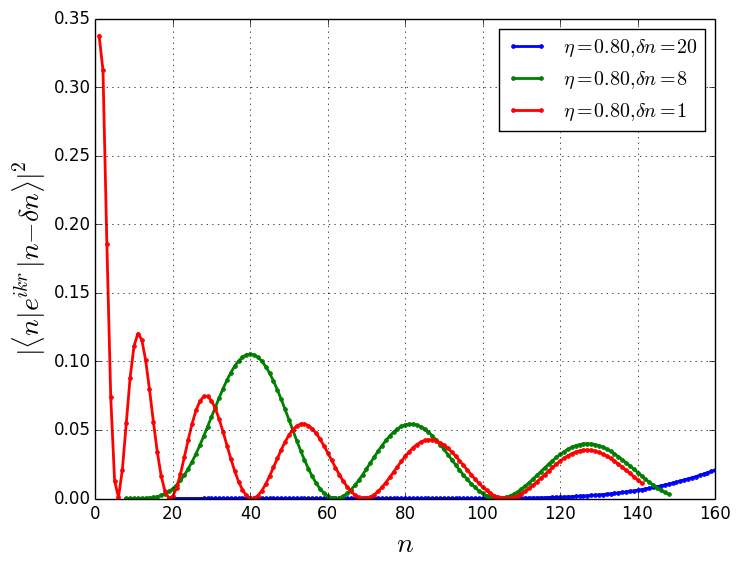
\includegraphics[width=7cm]{../raman_0.8_1.png}
  \end{center}
  \caption{Coupling strength to lower vibrational state for different initial states.}
  \label{fig-raman-curve}
\end{figure}
\begin{figure}
  \begin{center}
    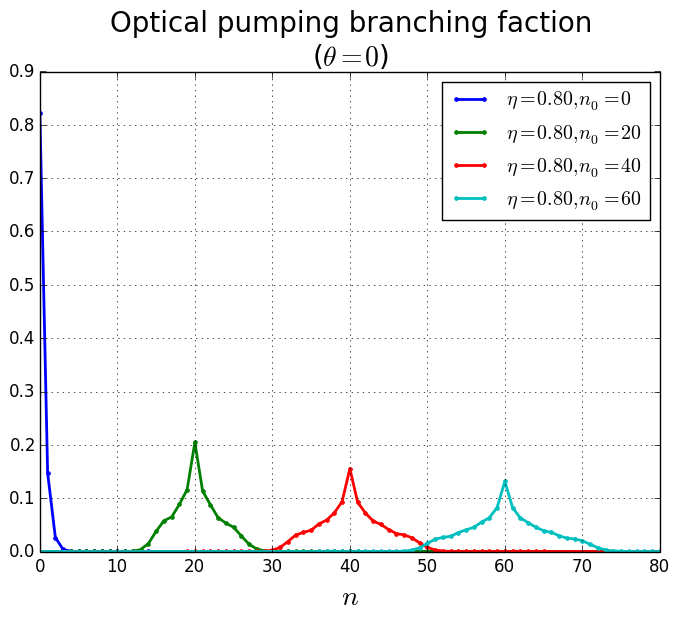
\includegraphics[width=7cm]{../pump_0.8_0_curve.png}
  \end{center}
  \caption{Possibilities of going in to other vibrational states (i.e. heating) during optical pumping for different initial level $n_0$. The pumping beam is sent in from the orthogonal direction.}
  \label{fig-pump-curve}
\end{figure}
\subsection{Calculations of the coupling coefficients}
In order to simulate the evolution of the system, it is necessary to calculate the strength of the sideband, i.e. the coupling between different vibrational levels. For the Raman transition, this can be directly calculated from equation \ref{lamb-dicke} and the result is shown in figure \ref{fig-raman-curve}. As we can see, due to the large Lamb-Dicke factor, there is significant coupling to lower vibrational state even for $\delta n$ as large as $8$.\\

For the optical pumping, since the scattered photon does not have a defined wave vector, in order to calculate the coupling to the vibrational states, one need to average over all different directions of the scattered photon. For pumping along the radial direction, the couplings between vibrational states are,
\eqar{
  \frac{\Gamma_{n,n'}}{\Gamma}=&\frac{1}{4\pi}\int_{0}^{2\pi}\ud\varphi\int_{-\frac\pi2}^{\frac\pi2}\ud\theta\cos\theta\abs{\langle n|\ue^{\ui\eta\paren{a+a^\dagger}\sin\theta}|n'\rangle}^2\\
  =&\int_{0}^{1}\ud x\abs{\langle n|\ue^{\ui\eta\paren{a+a^\dagger}x}|n'\rangle}^2
}
where $\Gamma_{n,n'}$ is the pumping rate from state $n$ to $n'$, $\Gamma$ is the original pumping rate for free atoms, and $\eta$ the Lamb-Dicke factor for the light along the direction of the confinement. The result of the calculation is shown in figure \ref{fig-pump-curve}. We can see that the heating, i.e. spread in $n$, is greater for the less confined higher vibrational levels. Moreover, because of the average over scatterred photon direction, the atom still has a large possibility of staying in the state $n=0$ after optical pumping.

\begin{figure}
  \begin{center}
    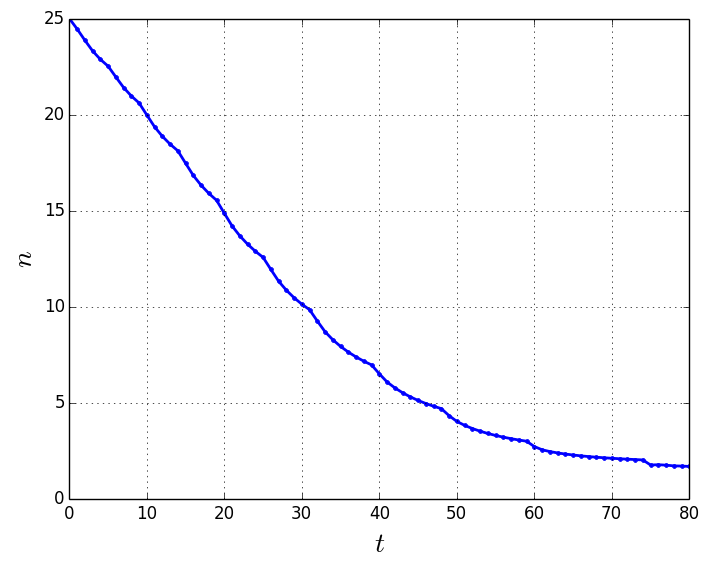
\includegraphics[width=7cm]{../n_decrease.png}
  \end{center}
  \caption{Decrease of $n$ during the cooling process.}
  \label{fig-n-decrease}
\end{figure}
\begin{figure}
  \begin{center}
    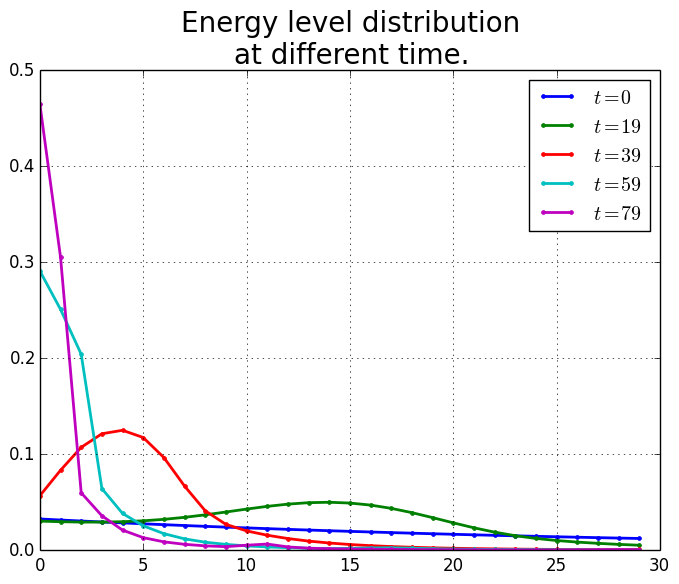
\includegraphics[width=7cm]{../cool_process.png}
  \end{center}
  \caption{Distribution in vibrational levels (including both hyperfine ground states) at different time. States with $n>30$ are not shown in the figure.}
  \label{fig-cool-process}
\end{figure}
\subsection{Evolution of the density matrix}
The evolution of the density matrix, including both the coherent Raman transition and the ``non-coherent'' optical pumping, is governed by the optical Bloch equation.
\eqar{
  \diff{\rho_{ij}}{t}=&-\frac12\sum_k\paren{\Gamma_{ki}+\Gamma_{kj}}\rho_{ij}+\ui\sum_k\paren{\rho_{ik}\Omega_{kj}-\rho_{kj}\Omega_{ik}}\\
  \diff{\rho_{ii}}{t}=&\sum_k\rho_{kk}\Gamma_{ik}-\sum_k\Gamma_{ki}\rho_{ii}+\ui\sum_k\paren{\rho_{ik}\Omega_{ki}-\rho_{ki}\Omega_{ik}}
}
where $\Gamma_{ij}$ and $\Omega_{ij}$ are the pumping rate and the Rabi frequency of the Raman transition between states $i$ and $j$ respectively. Since in the weak coupling limit, i.e. when the off resonance coupling is negligible, the only two time scales are the $\Gamma$'s and $\Omega$'s, we normalize the maximum Rabi frequency to $1$ in the simulation.

\section{Results of the simulation}
The simulation of the Raman sideband cooling is done by minimizing the average vibrational levels after a certain time. The free parameters in the simulation are the $\delta n$ for the Raman transition and the relative rate of the optical pumping $\Gamma/\Omega$. In order to get a stable and reliable simulation result, the change of these parameters are limited to smooth functions, which are further limited to exponential decays in this simulation for simplicity.\\

The result of this simple optimization is a sequence with $\delta n$ decreases from $12$ to $2$ and with the optical pumping rate decreases from $2$ to $1$. Figure \ref{fig-n-decrease} shows the change in the average vibrational levels during the cooling process. We can clearly see that even if the Lamb-Dicke factor is large and we started with a high tempeature, the Raman sideband cooling with $\delta n\gg1$ can still efficiently cool the atom in the trap to $12$ times colder then the initial temperature. Figure \ref{fig-cool-process} is the energy level distribution at different time which shows that more than $75\%$ of the atoms are in the two lowest vibrational levels at the end of the cooling.

\section{Conclusion}
In this paper, I have shown with numerical simulation of the optical Bloch equation that Raman sideband cooling with $\delta n\gg1$ can be used to effeciently cool neutral atoms in a optical dipole trap with $\eta\approx1$ and high initial temperature. Future improvement of this might include automatic optimization of the sequence and also the simulation of cooling in all three dimensions.

\bibliography{paper}
\end{document}
